\documentclass[11pt,a4paper]{article}

\usepackage[utf8]{inputenc}
\usepackage[T1]{fontenc}
\usepackage[polish]{babel}
\usepackage{lmodern}
\usepackage[margin=2cm]{geometry}
\usepackage{graphicx}
\usepackage{booktabs}
\usepackage{ltablex}
\keepXColumns
\usepackage{enumitem}
\usepackage[hidelinks]{hyperref}

\setlist{nosep}
\graphicspath{{img/}}

\title{Cerio\\[0.3em]\large Stan projektu i podział pracy}
\author{Igor Maciejak 197838}
\date{22.10.2026}

\begin{document}

\maketitle

\subsection*{Funkcjonalności działające}
\begin{itemize}
  \item gra w~przeglądarce oraz w~trybie headless (Node.js), służącym do treningu bota,
  \item proceduralne generowanie poziomów z~segmentów; poziomy są generowane na podstawie seeda i~zawierają również jaskinie,
  \item rury prowadzące do jaskiń,
  \item większość przeciwników i~power-upów z~SMB1,
  \item monety, czerwone monety, ruchome platformy, niszczenie bloków,
  \item animowane sprite'y,
  \item prosta architektura sterująca graczem,
  \item sterowanie przeciwnikami z~zewnątrz oraz prosty RL nagradzający przeciwników za ruch w~stronę gracza.
\end{itemize}

\subsection*{Funkcjonalności w~toku}
\begin{itemize}
  \item sieć neuronowa oraz trening bota metodą RL i~algorytmem genetycznym,
  \item integracja z~serwerem w~języku Python,
  \item tworzenie map na podstawie SMB3,
  \item dodanie do map pozostałych przeciwników i~power-upów zaimplementowanych w~kodzie.
\end{itemize}

\begin{figure}[h!]
  \centering
  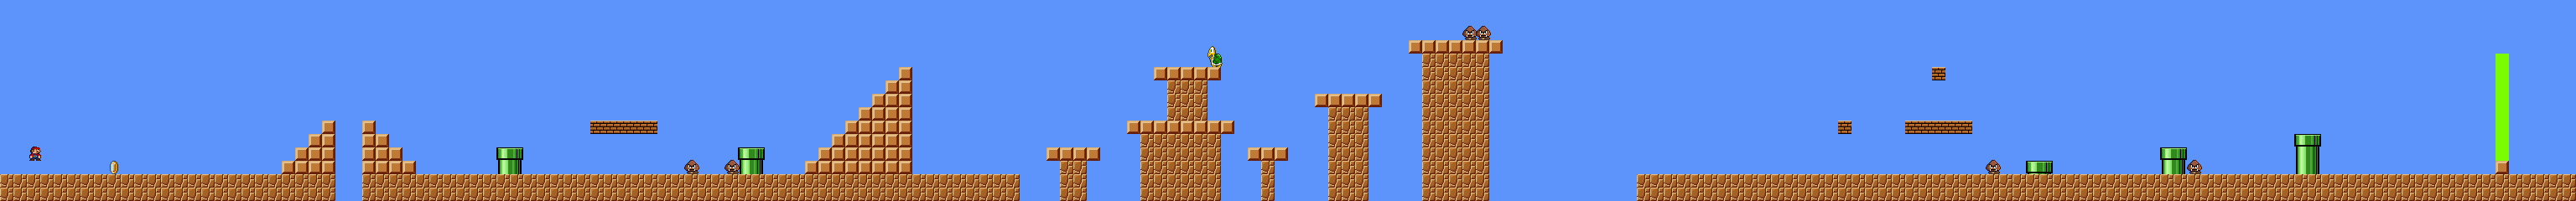
\includegraphics[width=\textwidth]{level_overworld.png}\\[0.5em]
  
\includegraphics[width=0.6\textwidth]{level_cave.png}\\[0.5em]
  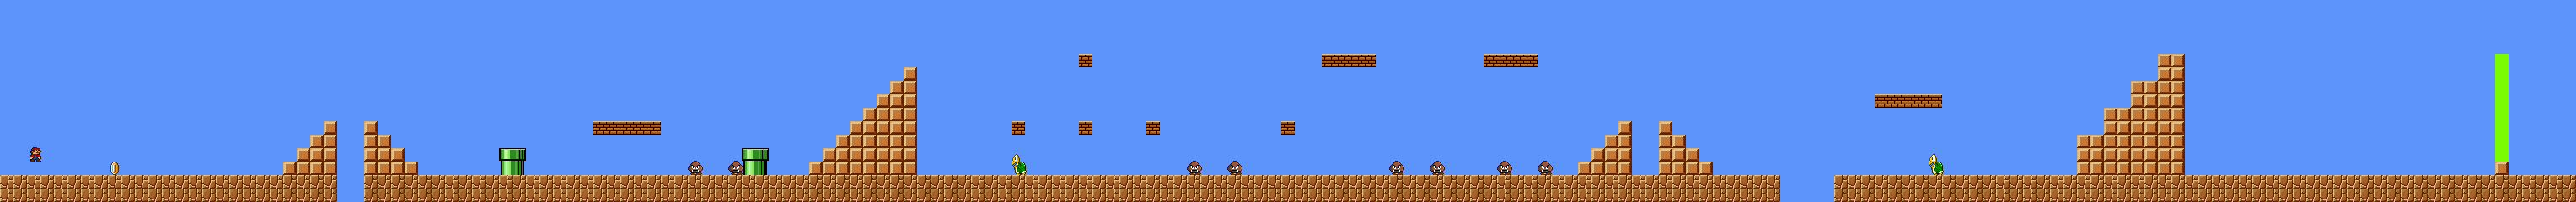
\includegraphics[width=\textwidth]{normal4_overworld.png}\\[0.5em]
  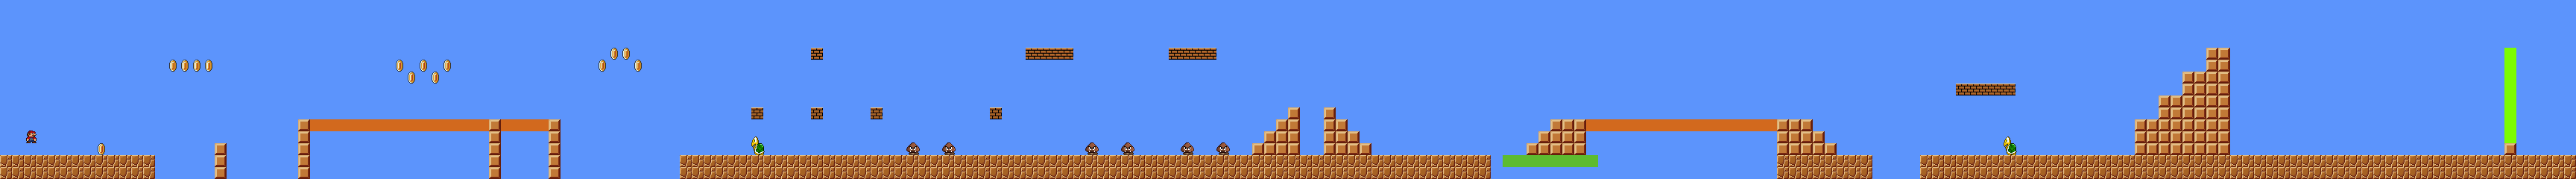
\includegraphics[width=\textwidth]{normal5_overworld.png}\\[0.5em]
  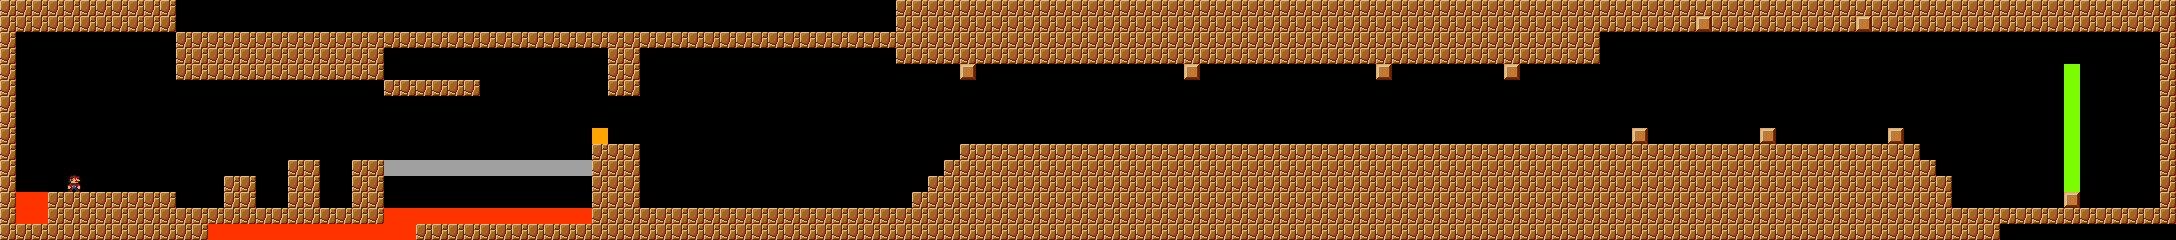
\includegraphics[width=\textwidth]{castle1_overworld.png}
  \caption{Przykładowe wygenerowane poziomy: normal z~jaskinią, dwa typu normal i~jeden typu castle.}
\end{figure}

\begin{figure}[h]
  \centering
  
\includegraphics[width=0.5\textwidth]{characters.png}
  \caption{Przykładowe sprite'y.}
\end{figure}

\newpage
\section{Podział prac w zespole}

\begin{tabularx}{\textwidth}{@{}>{\raggedright\arraybackslash}p{3.6cm} X@{}}
\toprule
\textbf{Osoba} & \textbf{Zakres prac} \\
\midrule
Igor Maciejak & Rdzeń gry, generator poziomów, rury i~jaskinie, niszczenie bloków, narzędzia diagnostyczne. \\
\addlinespace
Wojciech Milewski & Notacja i~normalizacja segmentów, poziomy normal, caves, castle. \\
\addlinespace
Albert Piątkowski & Pierwsze segmenty, monety i~czerwone monety. \\
\addlinespace
Jakub Piotrowicz & Przeciwnicy: Goomba, Koopa Paratroopa; ruchome platformy. \\
\addlinespace
Antoni Stępień & Przeciwnicy: Hammer Bro, Buzzy Beetle, Spiny, Bullet Bill, wieża Goomb. \\
\addlinespace
Filip Pawelec & Przeciwnicy: Koopa; mechanika power-upów oraz Star, Tanooki, Stopwatch, Leaf, Super Mushroom. \\
\addlinespace
Jan Nowosadzki & Przeciwnicy: Piranha Plant; power-upy Fire Flower i~Hammer, losowanie power-upów. \\
\addlinespace
Maria Szcześniak & Sprite'y i~animacje, wygląd jaskiń. \\
\addlinespace
Michał Mańkowski & Prosta architektura sterująca botem, sterowanie przeciwnikami z~zewnątrz i~prosty RL. \\
\bottomrule
\end{tabularx}

\section{Ocena}

\begin{tabularx}{\textwidth}{@{}p{3.6cm} c X@{}}
\toprule
\textbf{Osoba} & \textbf{Ocena} & \textbf{Uzasadnienie} \\
\midrule
Igor Maciejak     & --- & Kierownik projektu. \\
Wojciech Milewski & 5   & Baza poziomów i~notacja segmentów. \\
Antoni Stępień    & 4,5 & Pięciu przeciwników. \\
Filip Pawelec     & 4   & Większość power-upów. \\
Jakub Piotrowicz  & 4,5 & Ruchome platformy, przeciwnicy. \\
Maria Szcześniak  & 4,5 & Warstwa graficzna. \\
Albert Piątkowski & 5   & Monety, pierwsze segmenty. \\
Jan Nowosadzki    & 4   & Piranha Plant, dwa power-upy, losowanie. \\
Michał Mańkowski  & 4   & Architektura bota i~prosty RL. \\
\bottomrule
\end{tabularx}

\end{document}
